% =============================================================================
% Greeks Bearing Nets — CSCI 1470 Final Project Poster
% Beamerposter, 48" x 36" landscape (4:3)
% Build: pdflatex poster.tex
% =============================================================================
\documentclass[final,t]{beamer}
\usepackage[size=custom,width=121.92,height=91.44,scale=1.15]{beamerposter}
\usepackage[utf8]{inputenc}
\usepackage[T1]{fontenc}
\usepackage{lmodern}
\usepackage{graphicx}
\usepackage{booktabs}
\usepackage{array}
\usepackage{amsmath,amssymb}
\usepackage{xcolor}
\usepackage{tikz}

\graphicspath{{../results/figures/}{./figures/}}

% --- Brown-ish palette ---
\definecolor{brunopri}{RGB}{79,17,17}     % deep crimson
\definecolor{brunosec}{RGB}{200,140,40}   % warm gold accent
\definecolor{brunobg}{RGB}{248,244,236}   % warm off-white
\definecolor{rulegray}{RGB}{120,120,120}

\setbeamercolor{background canvas}{bg=brunobg}
\setbeamercolor{block title}{fg=white,bg=brunopri}
\setbeamercolor{block body}{fg=black,bg=white}
\setbeamerfont{block title}{size=\large,series=\bfseries}
\setbeamertemplate{navigation symbols}{}
\setbeamertemplate{itemize items}{\color{brunopri}\textbf{--}}

% Tighter blocks
\setbeamertemplate{block begin}{
  \begin{beamercolorbox}[wd=\textwidth,ht=2.4ex,dp=0.6ex,leftskip=0.6em,rightskip=0.6em]{block title}
    \insertblocktitle
  \end{beamercolorbox}
  \begin{beamercolorbox}[wd=\textwidth,leftskip=0.7em,rightskip=0.7em,vmode]{block body}
    \vspace{0.3em}
}
\setbeamertemplate{block end}{\vspace{0.3em}\end{beamercolorbox}\vspace{0.6em}}

% =============================================================================
\title{\Huge\textbf{Greeks Bearing Nets}\\[0.25em]
       \Large Synthetic Markets and Transformer Pricing for SPY Options}
\author{CSCI 1470 -- Deep Learning Final Project}
\institute{Brown University \quad \textbar \quad Spring 2026}
\date{}

\begin{document}
\begin{frame}[t]

% --- Header bar ---
\begin{center}
\begin{tikzpicture}
  \fill[brunopri] (0,0) rectangle (\paperwidth,3.2);
  \node[white] at (\paperwidth/2, 2.1) {\fontsize{60}{72}\selectfont\textbf{Greeks Bearing Nets}};
  \node[brunosec] at (\paperwidth/2, 0.85) {\fontsize{28}{34}\selectfont\textbf{Synthetic Markets and Transformer Pricing for SPY Options}};
\end{tikzpicture}\\[0.2em]
{\large CSCI 1470 -- Deep Learning Final Project \quad\textbullet\quad Brown University \quad\textbullet\quad Spring 2026}
\end{center}
\vspace{0.4em}

% =============================================================================
\begin{columns}[t,totalwidth=\paperwidth]

% =============================================================================
% COLUMN 1
% =============================================================================
\begin{column}{0.32\paperwidth}

\begin{block}{Motivation}
The Black-Scholes (BS) formula gives the textbook price of a European option,
but its assumption of constant volatility and Gaussian returns is famously
wrong: real markets exhibit a \emph{volatility smile}, fat tails, and
volatility clustering. We ask whether a deep model trained on
\textbf{synthetic market histories} can price options more faithfully than
BS, particularly in the regions where BS misprices most.
\vspace{0.2em}
\begin{itemize}
  \item \textbf{Goal.} Beat Black-Scholes on out-of-sample SPY option prices.
  \item \textbf{Idea.} Use a TimeGAN to generate realistic SPY price paths,
        then train a Transformer pricer on options simulated through those
        paths.
  \item \textbf{Test.} Compare against BS, a Heston-trained baseline, and
        a real-market regression on a held-out 2023--2024 sample.
\end{itemize}
\end{block}

\begin{block}{Data}
\begin{itemize}
  \item \textbf{Underlying.} SPY daily OHLCV, 2010--2024 (\(\sim\)3{,}500 days).
  \item \textbf{Options.} EOD SPY chain, 2023--2024 ($\sim$135K contracts after
        cleaning), with strike, expiry, mid-quote, IV, and BS Greeks.
  \item \textbf{Macro / market state.} VIX, 10Y yield, realized vol, term
        spread, returns at multiple horizons -- 20 features per day.
  \item \textbf{Sequences.} 30-day rolling windows of these 20 features feed
        the price-history encoder.
\end{itemize}
\vspace{0.2em}
\begin{center}
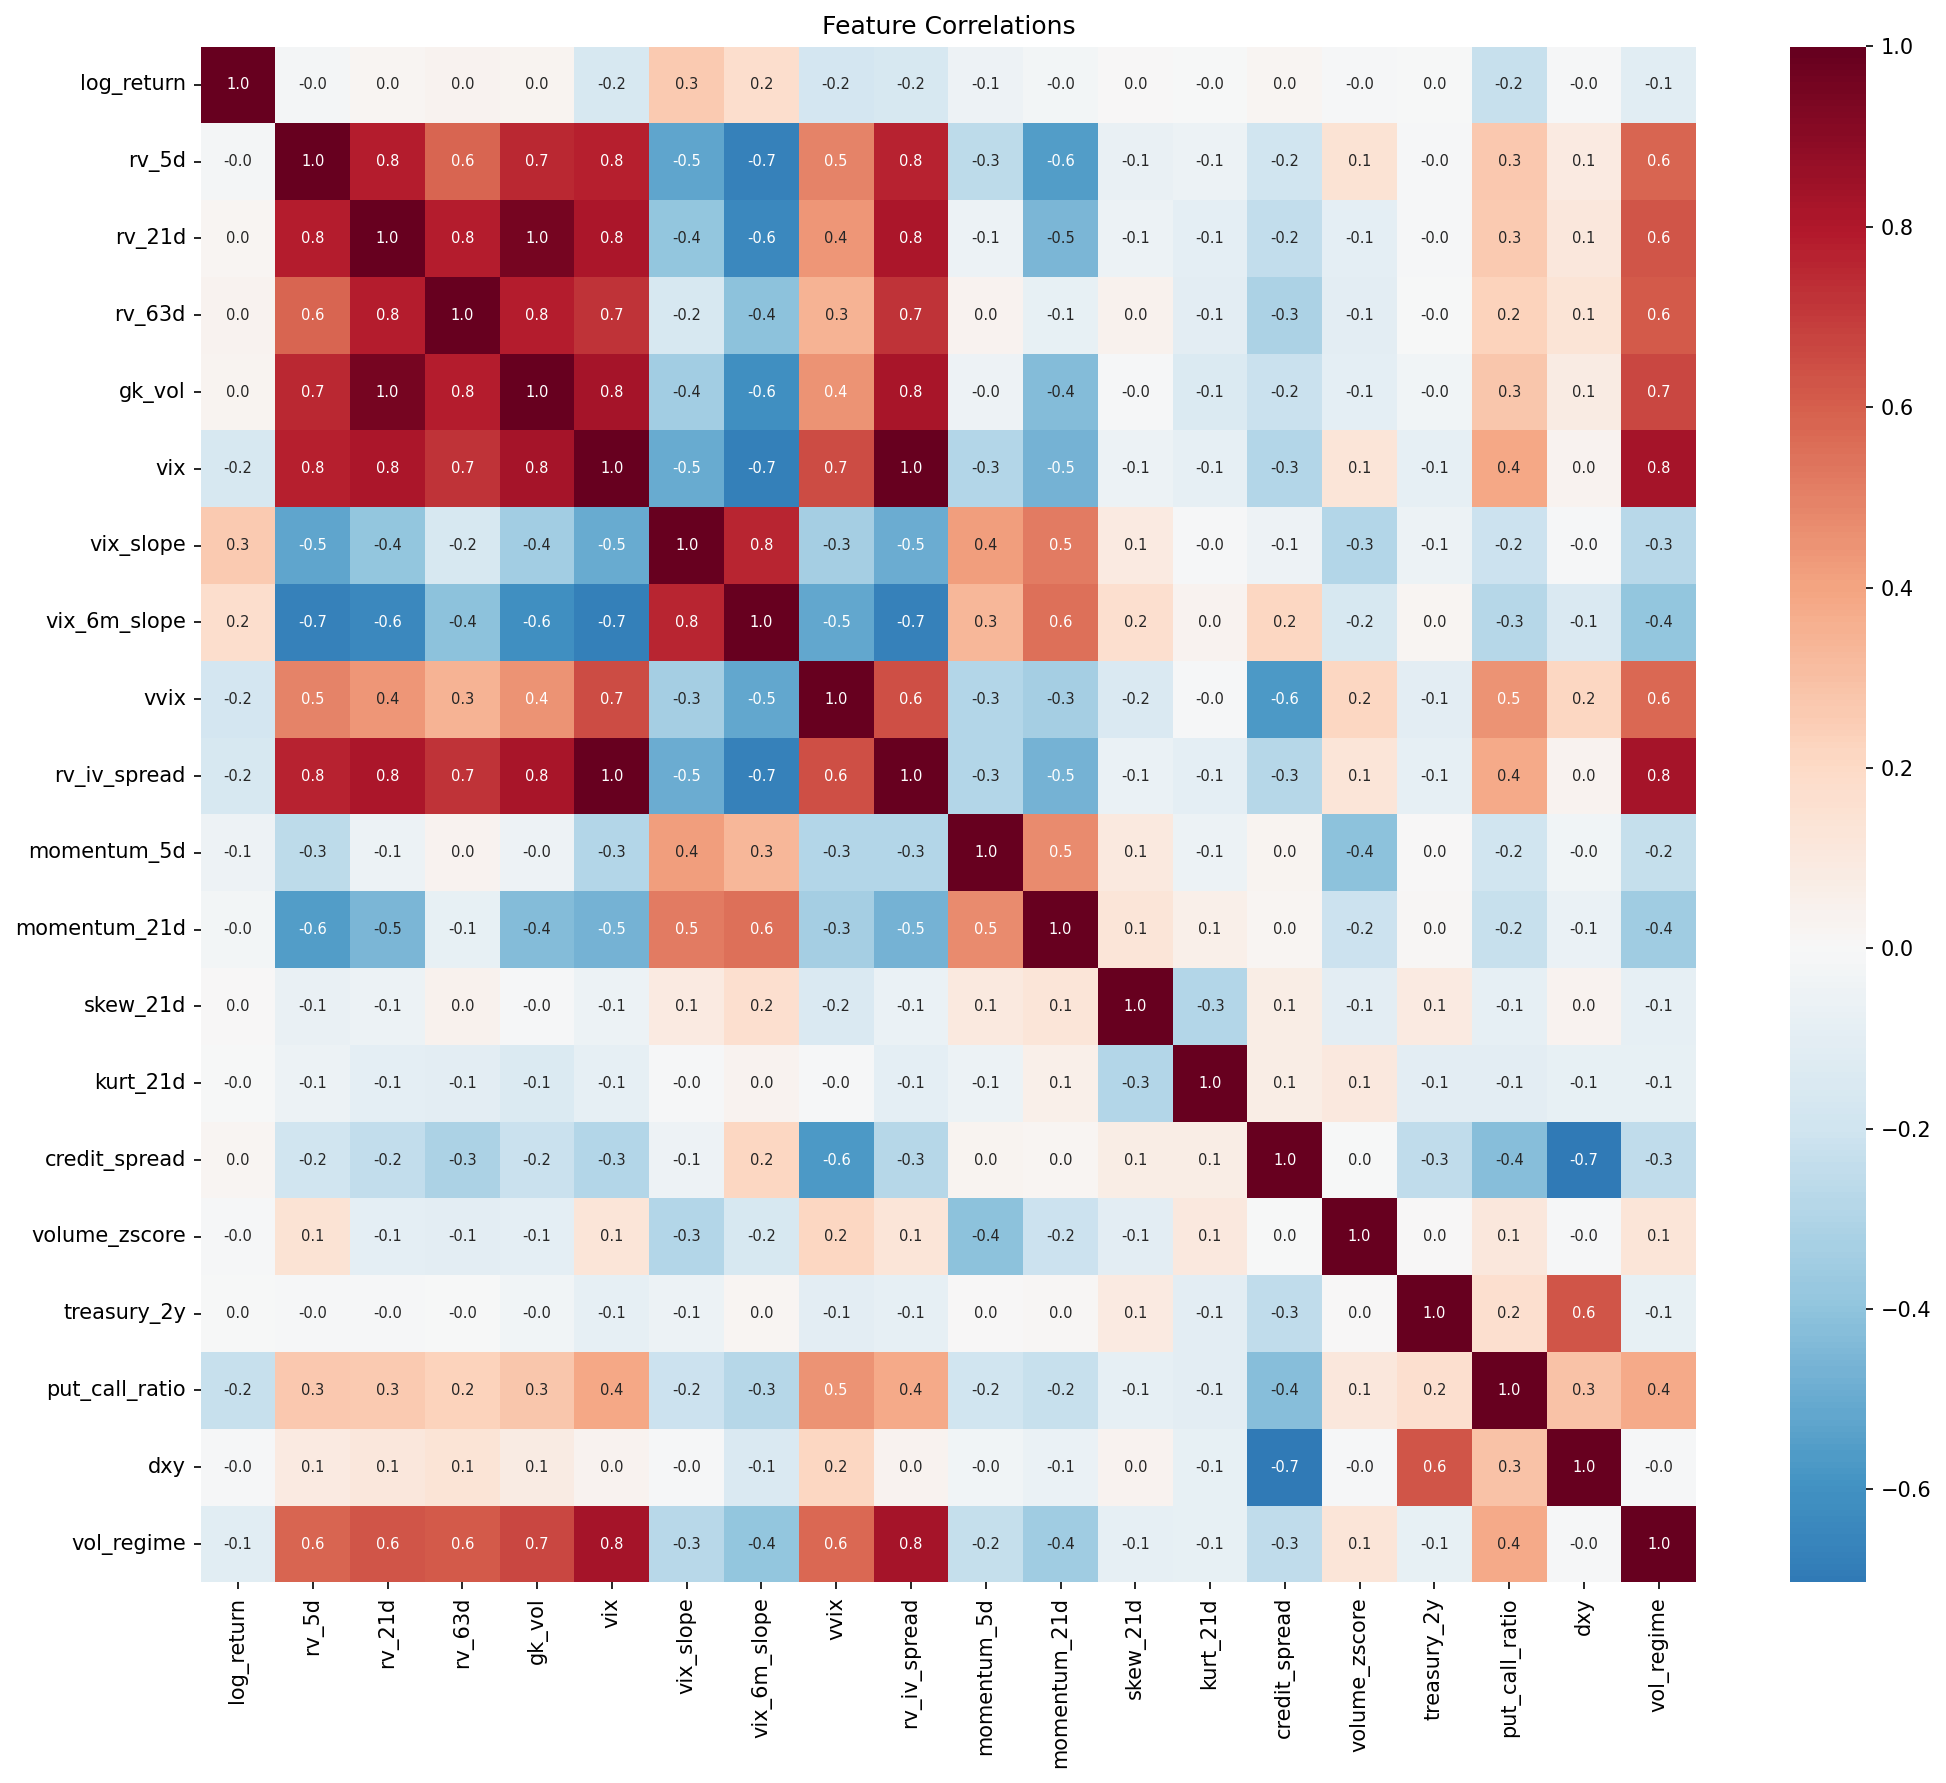
\includegraphics[width=0.95\linewidth]{eda_correlation.png}\\[0.1em]
{\small Feature correlation heatmap. VIX, realized vol, and short-horizon
returns carry the strongest signal for option mispricing residuals.}
\end{center}
\end{block}

\begin{block}{Black-Scholes Baseline}
\[
C_{\text{BS}} = S\,N(d_1) - K e^{-rT} N(d_2), \qquad
d_1 = \tfrac{\ln(S/K)+(r+\tfrac12\sigma^2)T}{\sigma\sqrt T}.
\]
We use \emph{realized} 20-day volatility for $\sigma$, the 10Y yield for $r$,
and contract-level $S$, $K$, $T$. This is the same input set our networks see,
so the comparison isolates the model, not the data.
\end{block}

\end{column}

% =============================================================================
% COLUMN 2
% =============================================================================
\begin{column}{0.34\paperwidth}

\begin{block}{TimeGAN: Learning the SPY Distribution}
TimeGAN (Yoon et al., 2019) couples an autoencoder with an adversarial game in
latent space, plus a supervisor that enforces step-to-step temporal
consistency. Five GRU sub-networks are trained in three phases:
\vspace{0.2em}
\begin{enumerate}
  \item \textbf{Phase 1.} Autoencoder pretraining: $\min \|R(E(x))-x\|^2$.
  \item \textbf{Phase 2.} Supervisor pretraining: predict next latent state.
  \item \textbf{Phase 3.} Joint adversarial training of $G$, $D$, $S$, with
        $E$/$R$ anchored on a reconstruction loss to keep the latent space
        well-defined.
\end{enumerate}

\textbf{Two fixes that mattered most.}
\begin{itemize}
  \item Dropping the final \texttt{Sigmoid} from $R$ -- the data is
        StandardScaler-normalized, so a $[0,1]$ output crushed every synthetic
        return positive and inflated GAN labels $4\times$.
  \item \texttt{BCEWithLogitsLoss} on linear $D$ logits -- the old
        \texttt{Sigmoid + BCE} combo saturated and triggered the runaway
        $G$-loss seen on Run 2.
\end{itemize}

\begin{center}
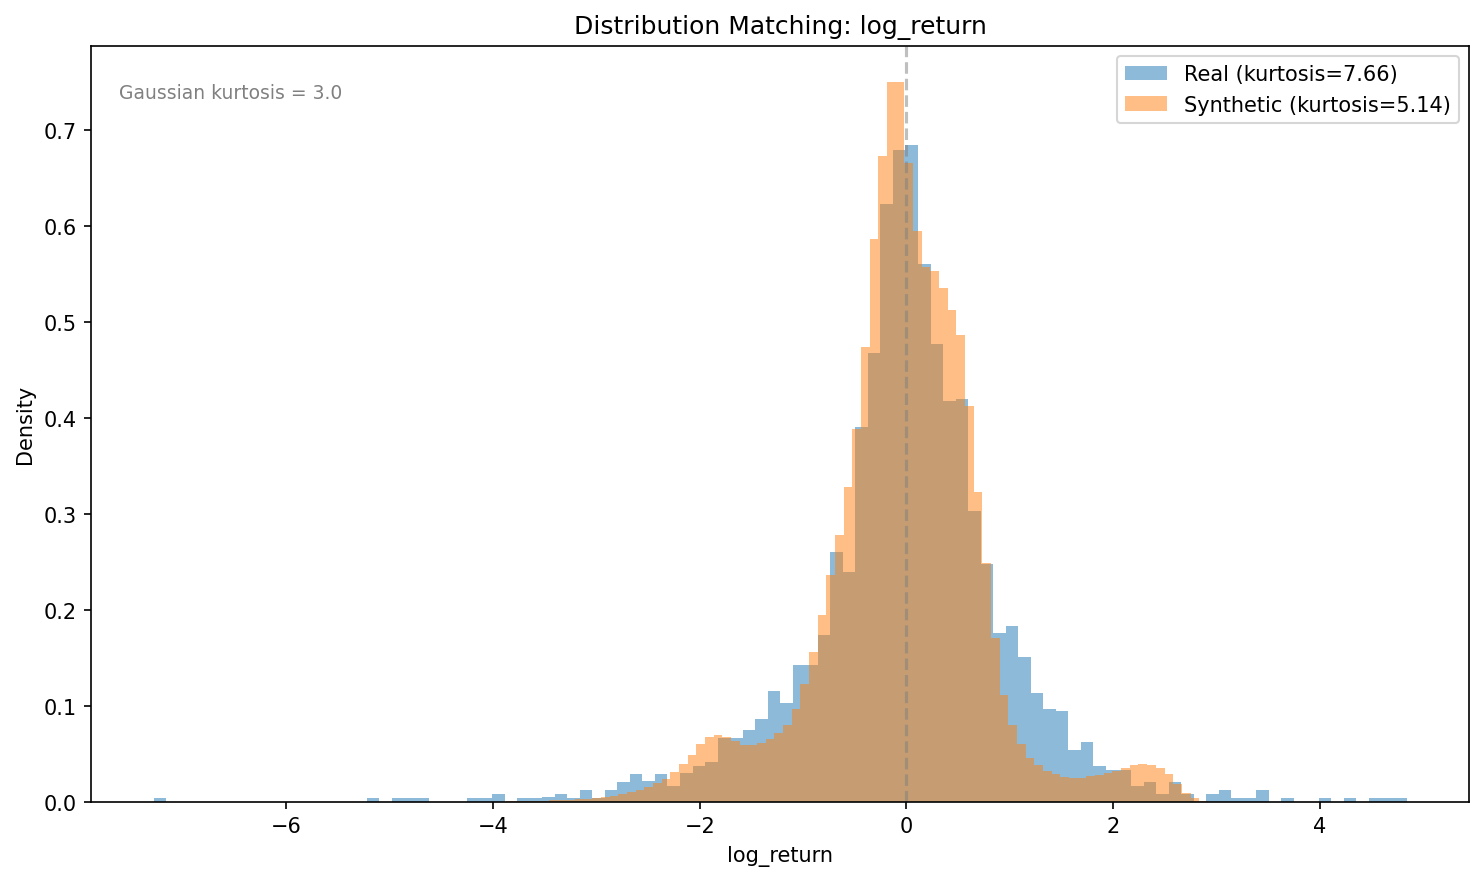
\includegraphics[width=0.95\linewidth]{gan_distribution.png}\\[0.1em]
{\small Real vs.\ synthetic 1-day log-returns. The GAN matches the variance,
the heavy tails, and the slight negative skew characteristic of equity
indices -- the structure BS explicitly throws away.}
\end{center}
\end{block}

\begin{block}{Transformer Pricer}
A single architecture, three label sources. Inputs:
\begin{itemize}
  \item A \textbf{30-day price-history sequence} (20 features) encoded by a
        4-layer Transformer encoder ($d_\text{model}{=}128$, 8 heads).
  \item An \textbf{8-feature contract block} ($S$, $K$, $T$, $r$, IV, $K/S$,
        $\log T$, BS-price input) projected and fused with the encoded
        history.
\end{itemize}
The head predicts $\log(\text{time value} + 1)$ -- training in log-space
killed the dead-ReLU collapse we saw on Run 2 and removed the need for an
output clamp.
\vspace{0.2em}
\begin{center}\small
\begin{tabular}{ll}
\toprule
\textbf{Variant} & \textbf{Training labels} \\
\midrule
A. Heston       & MC pricing under a fitted Heston SV model \\
B. GAN (RN)     & MC pricing on 2{,}000 GAN paths, \emph{risk-neutral drift} \\
C. Mixed + ATM  & 50/50 Heston + GAN-RN, ATM-weighted sampling \\
\bottomrule
\end{tabular}
\end{center}
\textbf{Why the RN correction matters.} TimeGAN learns the physical measure
$P$ of SPY, but options are priced under the risk-neutral measure $Q$. We
apply a per-step Girsanov shift $r/252 - \tfrac12\sigma_t^2 - \mu_{P,t}$ when
generating GAN-based labels; without it the GAN's positive equity drift bled
straight into mispriced calls.
\end{block}

\end{column}

% =============================================================================
% COLUMN 3
% =============================================================================
\begin{column}{0.32\paperwidth}

\begin{block}{Results: 2023--2024 SPY Options}
\textbf{C beats Black-Scholes overall} on both MAE and MSE; A is essentially
tied with BS on MAE while halving MSE on long-dated tails; B underperforms.
\vspace{0.2em}
\begin{center}\footnotesize
\setlength{\tabcolsep}{4pt}
\renewcommand{\arraystretch}{1.05}
\begin{tabular}{lcccc}
\toprule
\textbf{Model} & \textbf{Overall} & \textbf{ITM} & \textbf{ATM} & \textbf{OTM} \\
\midrule
Black-Scholes        & 1.515         & 1.44          & \textbf{1.58} & 1.54 \\
Transformer A (Heston)  & 1.552         & 1.24          & 2.10          & \textbf{1.17} \\
Transformer B (GAN, RN) & 2.148         & 1.62          & 2.75          & 2.06 \\
Transformer C (Mixed)   & \textbf{1.510}$^\star$ & \textbf{1.18} & 1.92 & 1.39 \\
\bottomrule
\end{tabular}\\[0.2em]
{\small MAE in dollars on held-out 2023--2024 contracts. \textbf{Bold} =
best per column; $\star$ = best overall.}
\end{center}

\vspace{0.4em}
\textbf{Where each model wins.}
\begin{center}\footnotesize
\setlength{\tabcolsep}{4pt}
\begin{tabular}{lcccc}
\toprule
\textbf{Slice} & \textbf{BS} & \textbf{A} & \textbf{B} & \textbf{C} \\
\midrule
Low VIX ($<$15)   & \textbf{0.81} & 1.49 & 1.78 & 1.59 \\
Med VIX (15--25)  & 1.24          & \textbf{1.04} & 1.80 & 1.15 \\
High VIX ($>$25)  & 2.21          & 2.49 & 2.89 & \textbf{2.13} \\
\midrule
Short expiry      & \textbf{1.09} & 1.27 & 1.89 & 1.26 \\
Medium expiry     & 1.82          & 1.86 & 2.17 & \textbf{1.76} \\
Long expiry       & 2.84          & 2.21 & 3.28 & \textbf{2.14} \\
\bottomrule
\end{tabular}
\end{center}
\vspace{0.2em}
{\small BS owns the easy regime (low vol, short expiry, ATM). The mixed
Transformer C dominates exactly the regions where BS structurally fails:
\textbf{long-dated, ITM, and high-volatility} contracts -- the smile.}
\end{block}

\begin{block}{What we learned}
\begin{itemize}
  \item \textbf{Mixing real-physics (Heston) and learned-distribution (GAN)
        labels works.} Each label source is a flawed teacher; together they
        regularize each other.
  \item \textbf{Smile capture is the win.} BS prices ATM near-perfectly --
        the model edge comes entirely from tails and tenor, not from the
        ``flat'' part of the surface.
  \item \textbf{The risk-neutral drift correction is non-optional.} Without
        it, the GAN-trained Transformer prices calls too high by construction.
  \item \textbf{Pure GAN labels (B) are not enough.} The GAN captures
        marginals well but its 60-day rollouts are noisier than Heston's
        analytic dynamics, so unmixed GAN labels add variance without
        structure.
\end{itemize}
\end{block}

\begin{block}{Limitations \& Future Work}
\begin{itemize}
  \item \textbf{MAPE is misleading on OTM.} OTM denominators are
        \$0.30--\$2, so a single dollar of error reads as 100\%+. We report
        MAE/MSE bucket-wise and quote MAPE only on ITM (where it is
        meaningful: \(\sim\)4--6\%).
  \item Single underlying (SPY) and a 2-year test window. Extending to
        multi-asset and to crisis years (2008, 2020) is the natural next test.
  \item No Greeks-level evaluation yet -- delta/vega-aware loss is the
        clearest path to using these models for hedging, not just pricing.
\end{itemize}
\end{block}

\begin{block}{}
\centering\small
Code \& data: \texttt{github.com/dma2459/greeks-bearing-nets}
\end{block}

\end{column}

\end{columns}
\end{frame}
\end{document}
